\vspace{-0.2cm}
\section{Introduction}
\vspace{-0.1cm}

\label{sec:introduction}



World Action Models (WAMs) aim to answer a coupled physical question:
\emph{given a task instruction, what motion should the robot execute,
and how will that motion change the surrounding world?}
Most existing WAMs couple action learning with prediction of future
images or visual latents, increasingly building on pretrained video models
\citep{yang2023unisim,li2025uva,zhu2025uwm,cen2025worldvla,
bi2025motus,ye2026dreamzero,yuan2026fastwam,zhou2026tau0wm}.
Robotic interaction, however, takes place in metric three-dimensional
space, and an image is only a view-dependent projection of that space.

The same robot motion, object displacement, or contact event can produce
different pixel changes across views, and equal pixel displacements
need not correspond to equal physical distances
\citep{ze2024threediffusion,qu2025spatialvla}.
Differences in camera intrinsics and camera-to-robot poses further
make this mapping vary across embodiments.
Evaluations of video-based WAMs report sensitivity to viewpoint and
robot-state changes \citep{zhang2026wamgeneralization}, and a
photorealistic prediction may still misrepresent object displacement,
deform rigid geometry, or allow static regions to drift
\citep{huang2026pointworld}.
Such visual representations leave metric motion and contact relationships
implicit for spatial reasoning, prediction, and control.

Recent methods incorporate depth, optical flow, scene flow, or
reconstructed 4D geometry into prediction
\citep{zhen2025tesseract,guo2026xwam,zhao2026rynnworld,wang2026lamp}
or ground action generation in explicit 3D structure
\citep{shridhar2023peract,ze2024threediffusion,zhen2024threedvla,
qu2025spatialvla}.
Yet geometry often serves as an input cue or auxiliary prediction target,
rather than a shared interface for action generation and scene dynamics.
PointWorld~\citep{huang2026pointworld} directly predicts metric point
flows conditioned on externally supplied robot motion, rather than
generating that motion from a task instruction.
A 3D-native WAM should place observations, actions, and resulting scene
changes in a shared metric frame, enabling task-conditioned behavior,
consequence prediction, and executable control.

We introduce \method{}, \textbf{UNI}fied \textbf{T}rajectories for
\textbf{A}ction and \textbf{S}cene flow.
To our knowledge, it is the first 3D-native world action model that
aligns observations, actions, and scene dynamics in a shared metric
frame within each prediction window, using a common representation
across robot embodiments and human hands, as illustrated in
Fig.~\ref{fig:physwam_overview}.

Realizing this 3D-native world action model presents three challenges.
First, visual observations must be grounded in metric space even
when depth is unavailable. We propose \emph{world-aligned 3D position embeddings} derived from observed depth or learned weights over
candidate positions along calibrated camera rays. Second, human hands and robot grippers have different morphologies
and control interfaces. We propose \emph{action flow}, which represents their motion as trajectories of corresponding 3D points in the shared frame. Third, trajectories differ in frame rate and duration across data sources. Representing each timestep as a token allocates backbone capacity
across unequal physical-time intervals. We propose a \emph{physical-time trajectory tokenizer}, which aligns each trajectory to elapsed time and encodes the whole trajectory as one token before the backbone.
\emph{Scene flow} describes scene-point displacements decoded from trajectory
tokens conditioned on action flow. 

In the backbone, observation tokens
are grounded in world coordinates, while action-flow tokens across
embodiments and scene-flow tokens are anchored at each point's current
3D position, allowing the network to model motion through features
associated with fixed spatial anchors.
Given the instruction and current observations, a layer-coupled
Mixture-of-Transformers jointly models point trajectories and executable
commands. This supports two modes: \emph{policy mode} directly generates
executable actions, while \emph{simulator mode} predicts scene changes
conditioned on externally supplied action flow.
A causal attention mask enables key--value caching of shared context
across denoising steps, reducing repeated computation and accelerating
inference.

% \emph{Scene flow} describes scene-point displacements that are decoded
% from trajectory tokens and conditioned on action flow. In the backbone, observation tokens, action tokens from different embodiments, and scene-flow tokens are all anchored only at the corresponding point's current 3D position, so the network only models how the point features in the current scene change.
% Consequently, given the instruction and the current observations, a layer-coupled Mixture-of-Transformers jointly models point trajectories and executable commands. We therefore provide two modes of use: \emph{policy mode} uses the generated motion, and \emph{simulator mode} replaces the action flow with an external one. A causal attention mask and a key-value cache allow the shared observation and language representation to be reused across rounds of action-flow and action-chunk generation, which speeds up inference. 


\begin{figure}
    \centering
    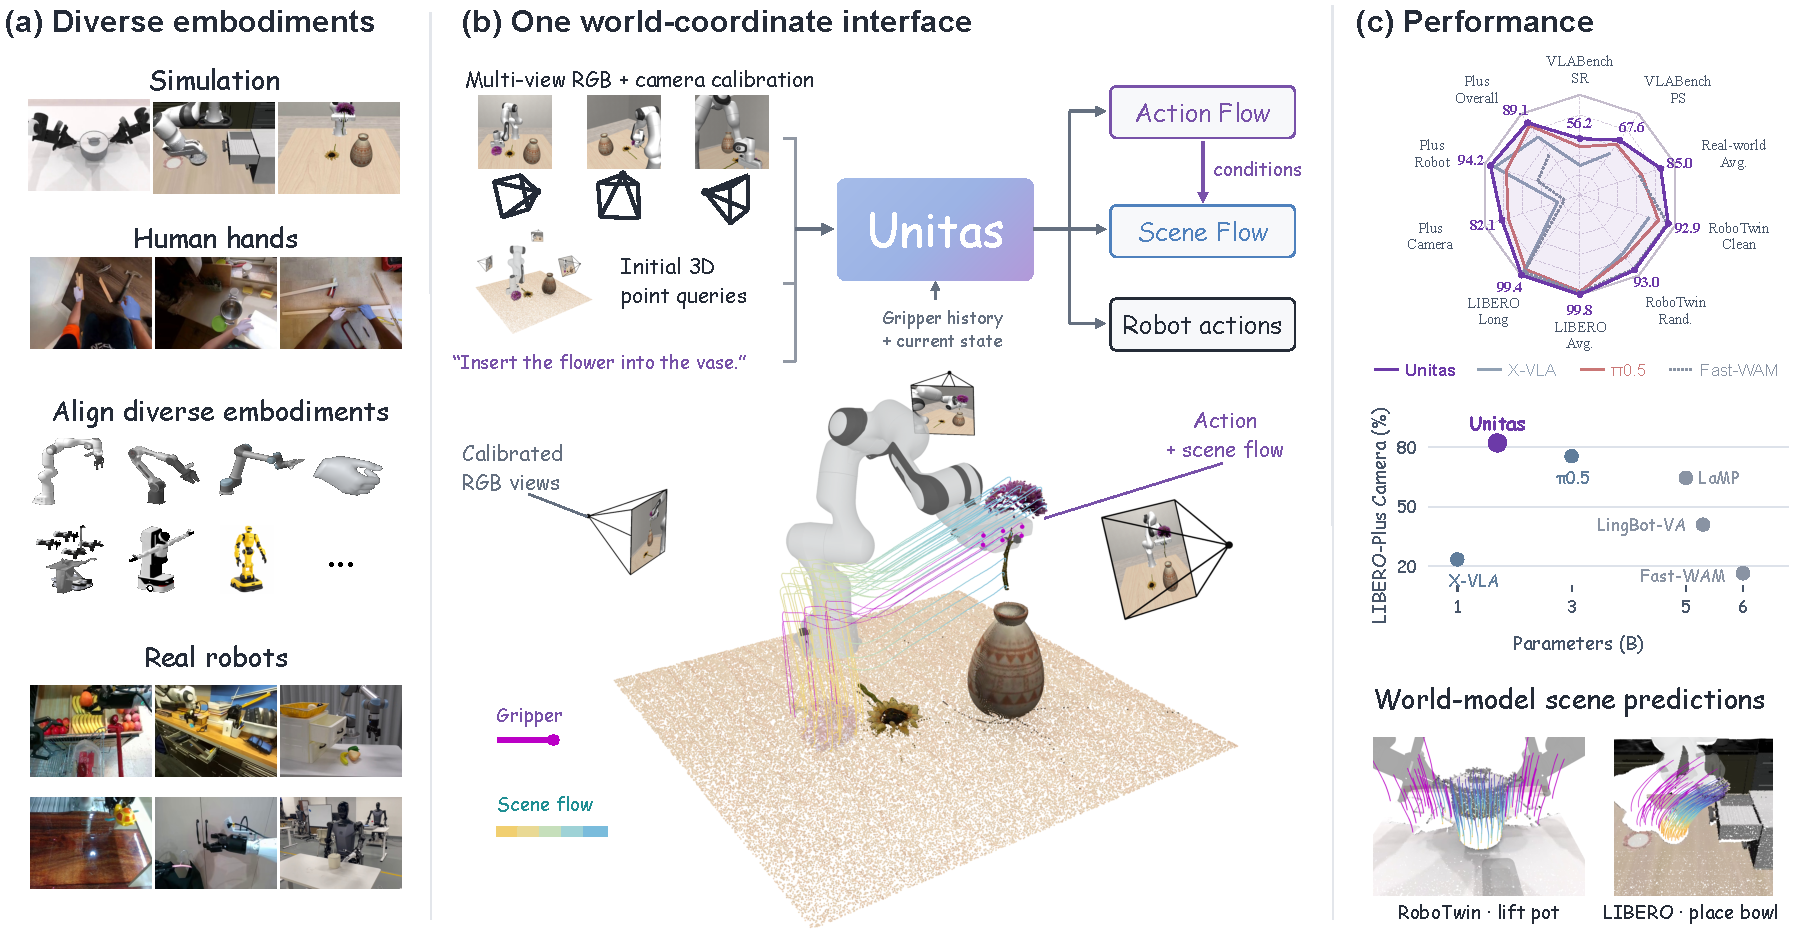
\includegraphics[width=\linewidth]{figures/unitas_overview.pdf}
    \vspace{-0.7cm}
    \caption{\textbf{\method{} is a 3D-native world action model.}
    Observations, action flow, and scene flow share a metric frame within
    each prediction window, with a common representation across embodiments.
    With 1.7B parameters, \method{} achieves leading manipulation results
    among the compared methods and predicts action-conditioned scene
    trajectories.\vspace{-0.4cm}}
    \label{fig:physwam_overview}
\end{figure}

We evaluate \method{} on action-conditioned scene prediction and
robotic manipulation.
In simulator mode, it leads the compared methods across all four
RoboTwin scene-prediction metrics, reducing Moving ADE, Moving FDE,
and Static ADE by 35\%, 21\%, and 49\%, respectively, relative to
PointWorld~\citep{huang2026pointworld}.
In policy mode, it achieves 99.8\% success on LIBERO and outperforms
larger video-based WAMs on RoboTwin.
It leads the compared methods in VLABench success rate and progress
score, and reaches 89.1\% success on LIBERO-Plus with strong robustness
to camera and robot-state changes.
Real-robot success reaches 90\% on \emph{Organize Books} and 65\% on
\emph{Pack the Ball}, exceeding both baselines.
Ablations show that world-aligned visual grounding, action- and scene-flow
supervision, and motion history improve policy performance and robustness.

Our contributions are:\nopagebreak[4]
\begin{itemize}
    \item To our knowledge, \method{} is the first 3D-native world action
    model that aligns observations, actions, and scene dynamics in a
    shared metric frame, using a common representation across robot
    embodiments and human hands.

    \item Action flow represents human hands and robot grippers through
    point trajectories, while scene flow represents the environmental
    response conditioned on that motion. Both policy and simulator modes
    use this interface.

    \item World-aligned positional embeddings ground visual observations
    with or without depth, and a physical-time trajectory tokenizer
    encodes each point trajectory as one token spatially anchored at its
    current 3D position.

    \item With 1.7B parameters, \method{} achieves leading action-conditioned
    scene prediction and strong manipulation performance in simulation
    and on real hardware.
\end{itemize}
